\section{How can we Slow down Aging?}

\subsection{Overview}

\begin{frame}[c]{Goal of Anti-Aging Research}
    \large
    As I understand it, the goal of anti-aging research is \textbf{the extension of the human lifespan}.

    Ideally by stopping aging or achieving neglegible senescence.
    Intermediate goals include slowing down aging, and increasing QUALYs (QUality-Adjusted-Life-Years).
\end{frame}

\begin{frame}[c]{Potential Strategies to Slow down Aging}
    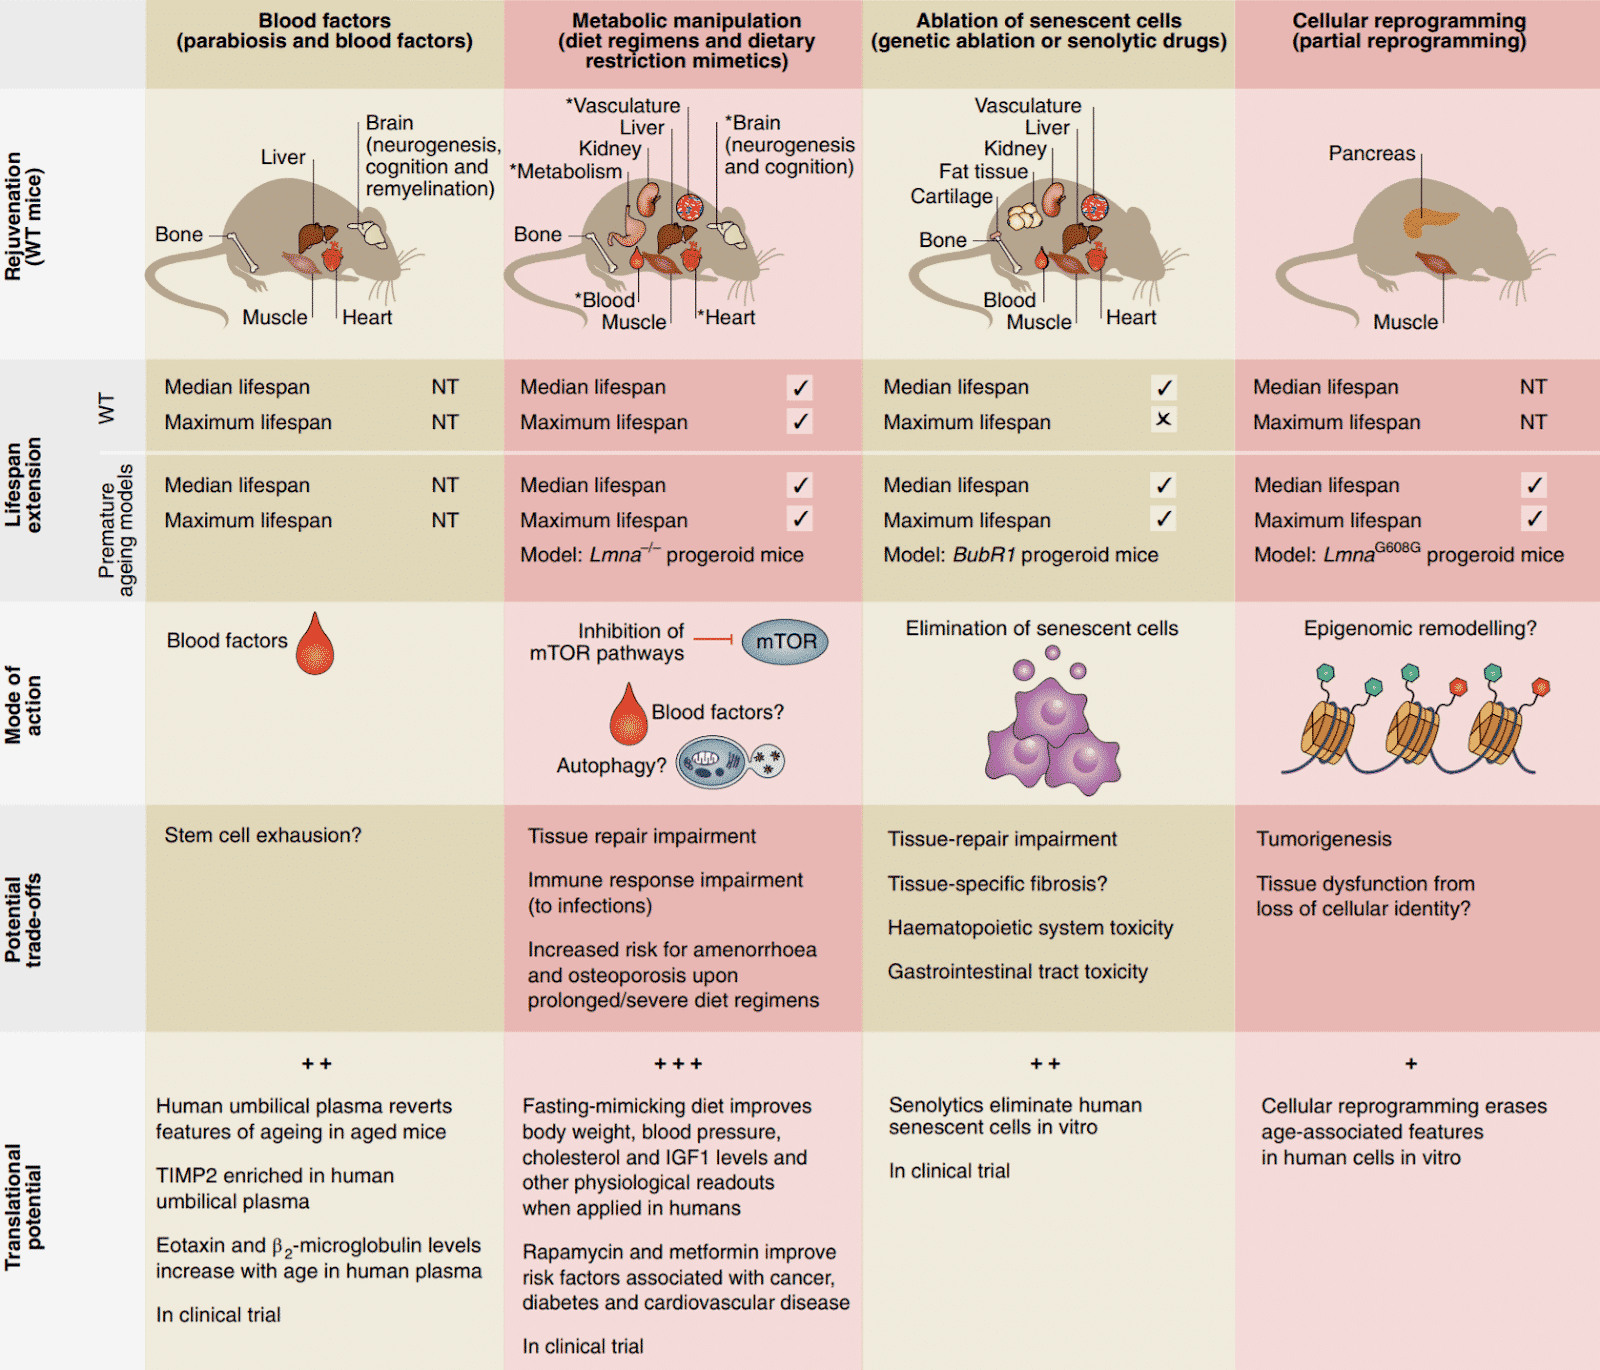
\includegraphics[height=0.85\textheight]{strategy_comparison} \\
    Source: \cite{mahmoudi2019turning}

    \pnote{A comparison of the four emerging rejuvenation strategies: blood factors,
    metabolic manipulation, ablation of senescent cells and cellular
    reprogramming. The figure depicts the features that improve when treatment
    in mice is initiated at midlife or later. The top panel shows organs or
    tissues that exhibit a rejuvenated phenotype in wild-type (WT) mice. For
    rapamycin, features that have been shown to improve also in young mice
    following treatment are indicated with an asterisk (*). The effect on
    lifespan, proposed primary mode (or modes) of action and possible
    trade-offs of these strategies are also presented. Finally, the
    translational potential in humans is indicated by the increasing number of
    plus signs (+) based on present evidence in human ageing and current
    feasibility. NT, not tested. Question marks indicate possible modes of
    action and trade-offs. Original source: \cite{mahmoudi2019turning}}
\end{frame}


\subsection{Parabiosis}

\begin{frame}[c]{Parabiosis (Blood Exchange)}
    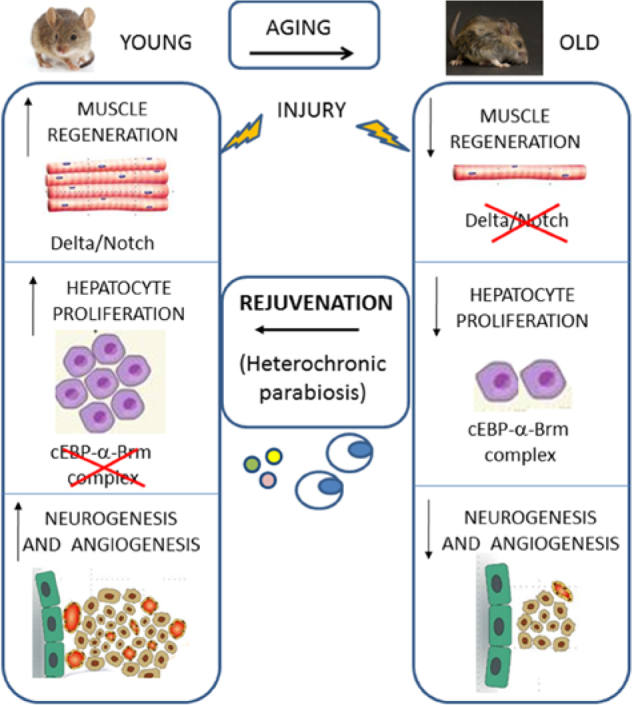
\includegraphics[height=0.85\textheight]{parabiosis_effects} \\
    Source: \cite{conese2017fountain}
\end{frame}

\begin{frame}[c]{Method Evaluation: Parabiosis}
    \large
    % Parabiosis (heterochronic parabiosis) is putting young blood into old mice, to make the old mice biologically younger. This is achieved in the lab by connecting the circulatory systems of young mice and old mice. Certain factors in the blood help to rejuvenate muscle, heart brain and liver tissues in old mice and restore their biological function.

% Equivalent procedures that modify the compounds within blood in humans such as apheresis (blood filtering) could be used to slow aging in humans and thereby prevent or slow the progression of many types of age-related diseases including Alzheimer's disease.

% Recently, a group of Russian biohackers recently took part in the first plasma dilution experiments in humans. In a research context, the safety and effectiveness of apheresis is being tested in a clinical trial in humans by the company Alkahest.

    \textbf{Hallmarks affected}:
    \begin{aquote}{\cite{conese2017fountain}}
        In principle, the heterochonic parabiosis reverts all phenotypic and molecular hallmarks of ageing by transferring soluble factors and cells.
    \end{aquote}
    % \begin{itemize}[<+(1)->]
    %     \item Stem cell exhaustion
    %     \item Cellular senescence
    %     \item Altered intercellular communication
    % \end{itemize}
    % parabiosis reverses age-related decline by targeting several hallmarks of aging including stem cell exhaustion, cellular senescence and altered intercellular communication (inflammation).

    \pause
    Alternatives: Blood Filtering and (Growth) Hormone Therapy. \\
    \pause
    \textbf{Status: In clinical trial}, e.g. \cite{AStudyto73:online}.
\end{frame}


\subsection{Metabolic Manipulation}

\begin{frame}[c]{Dietary Restriction in D. melanogaster (Fruit Fly)}
    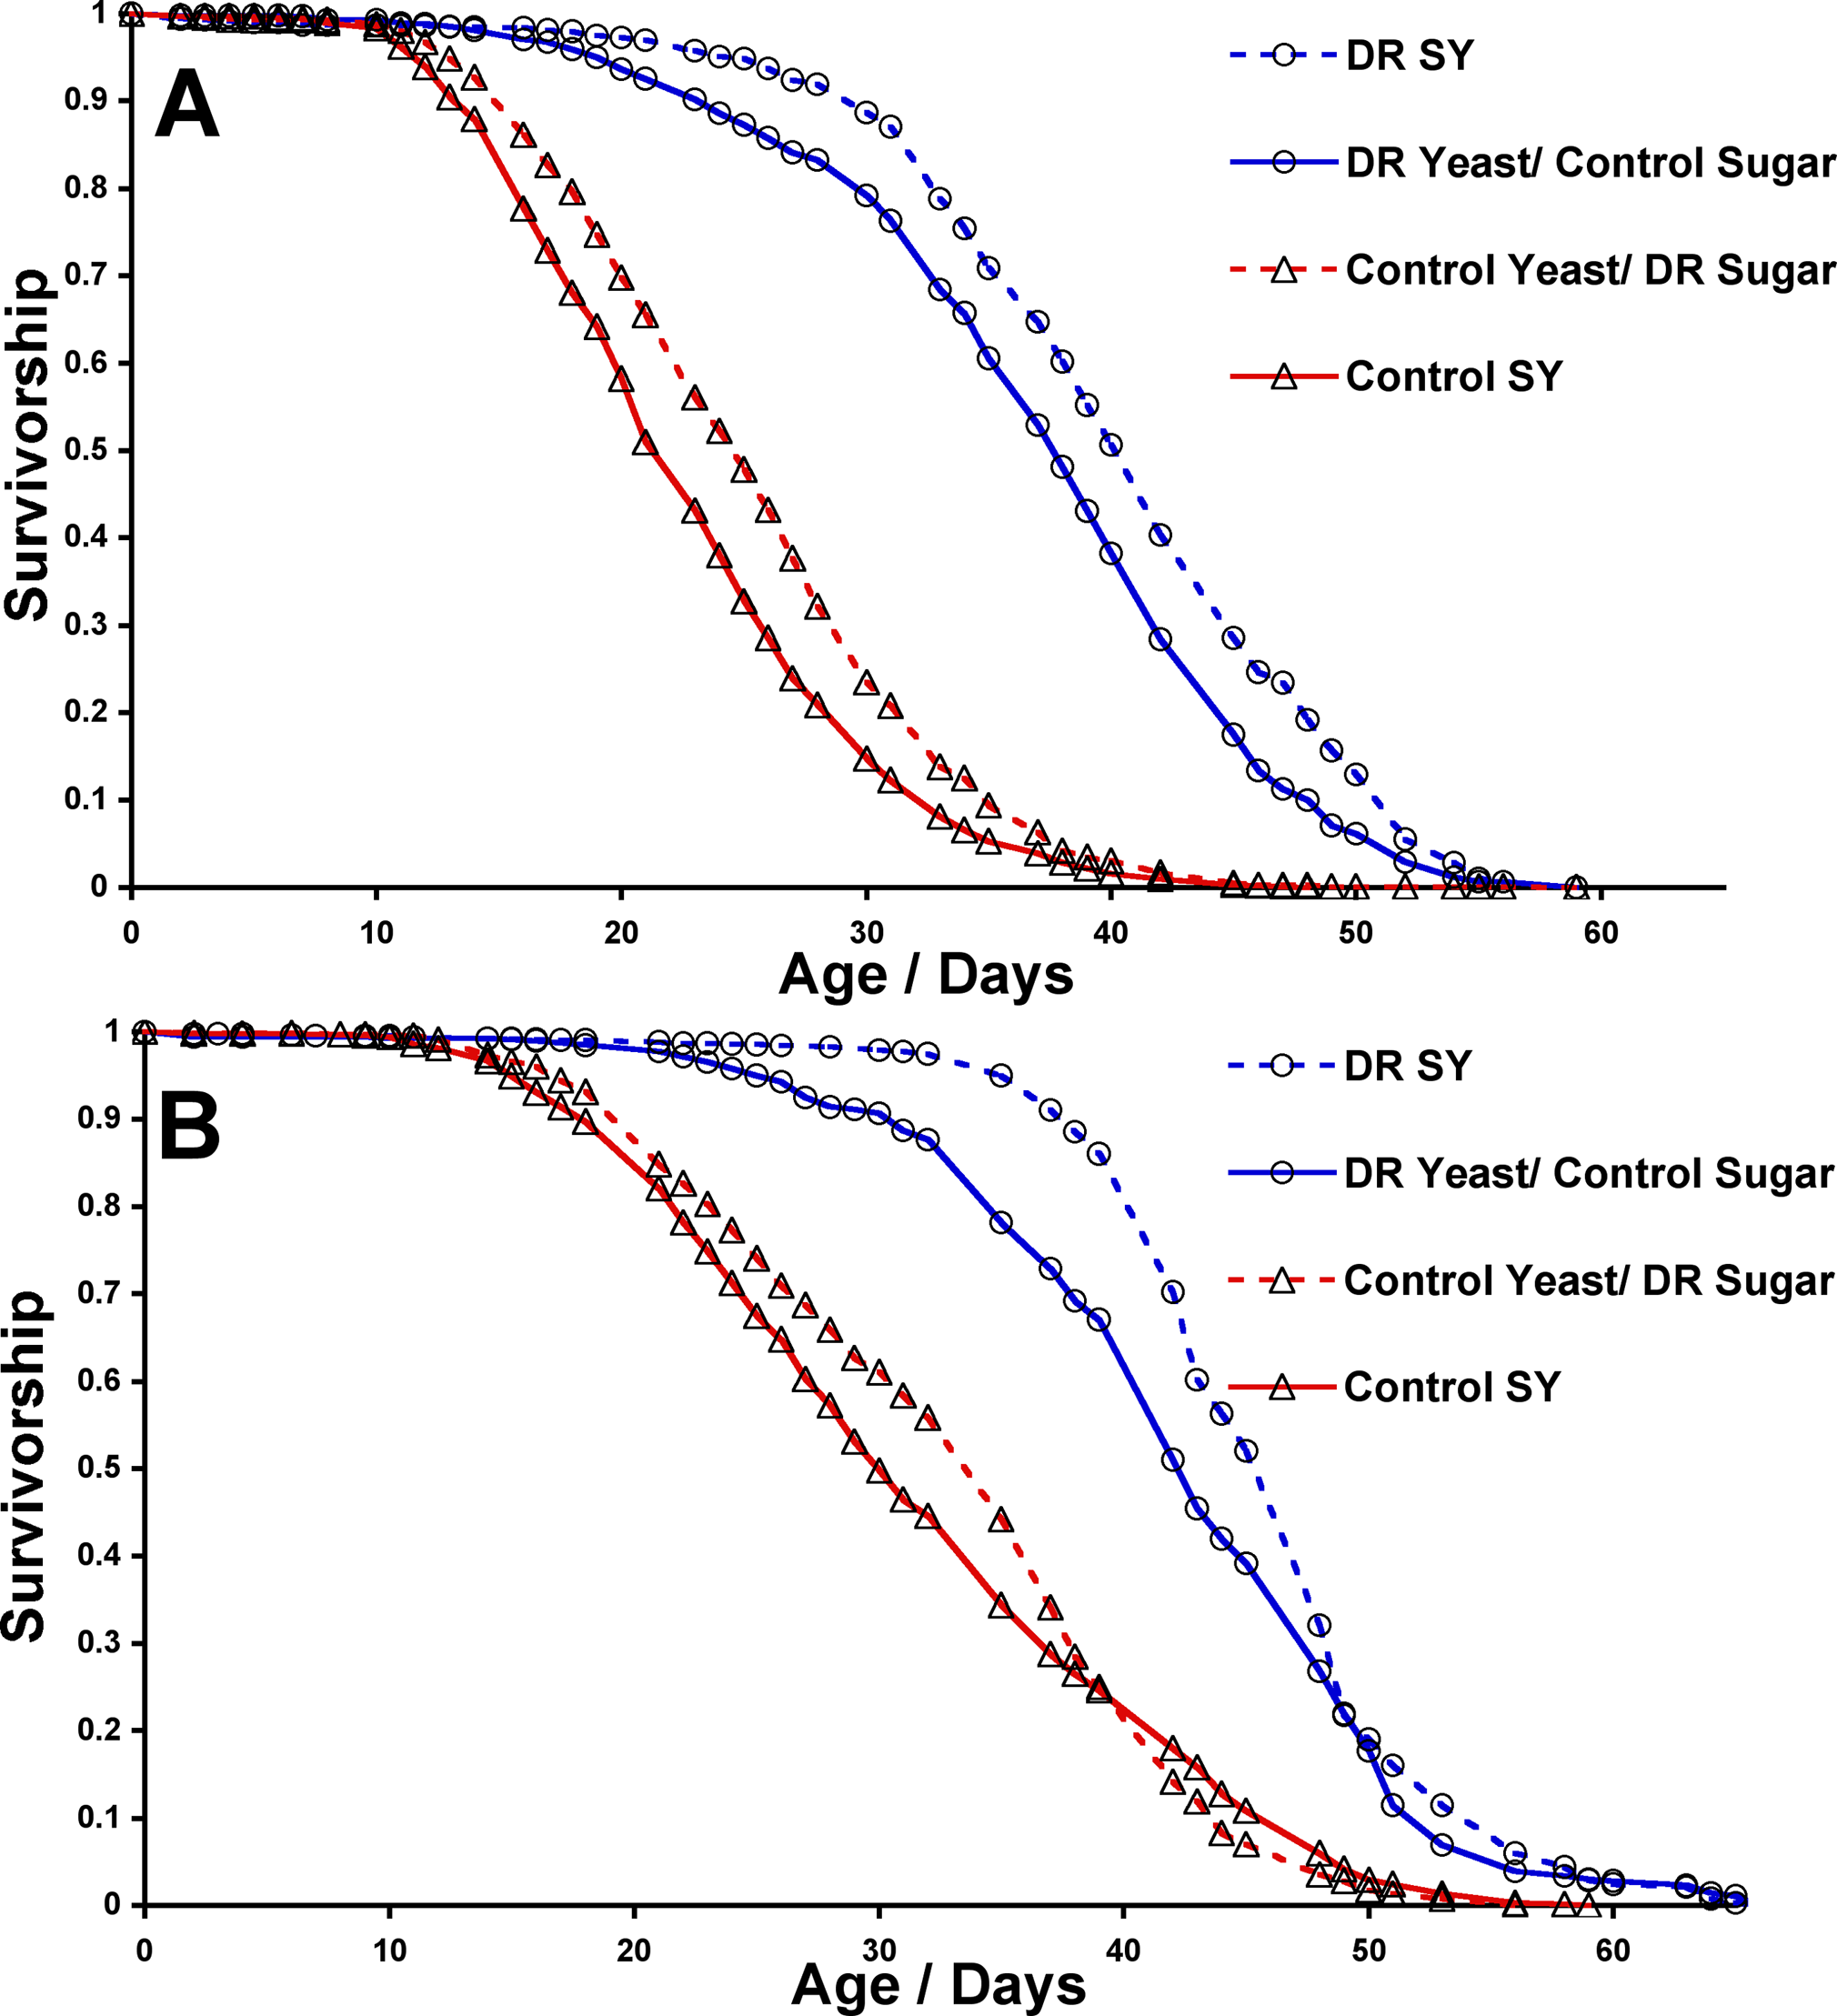
\includegraphics[height=0.85\textheight]{cr_lifespan_increase} \\
    Source: \cite{mair2005calories}
\end{frame}

\begin{frame}[c]{Dietary Restriction Pathways in Yeast}
    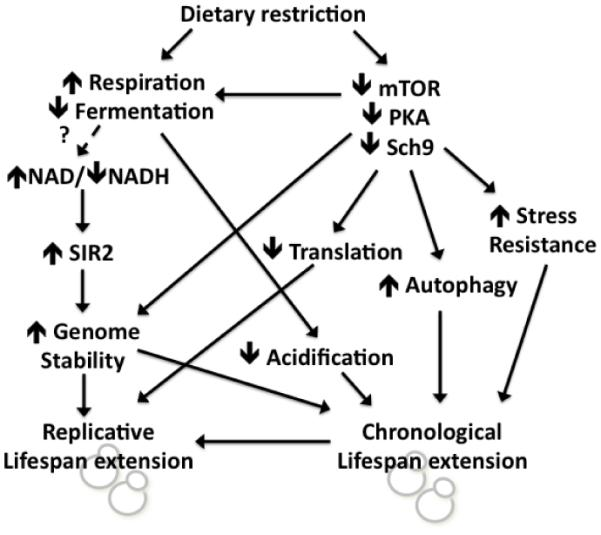
\includegraphics[height=0.85\textheight]{dietary_restrict_yeast} \\
    Source: \cite{kapahi2017dietary}
\end{frame}


\begin{frame}[c]{Dietary Restriction Effects}
    \large
    \begin{itemize}[<+(1)->]
        \item 'Different' mitochondrial energy production (less ROS)
        \item Increased repair capacity (SIRT and others)
        \item Increased removal of misfolded proteins
        \item Reduced intracellular (oxidative) stress
        \item Reduced inflammation and proliferation
    \end{itemize}
    Overall: Optimizing energy and resource usage
\end{frame}


\begin{frame}[c]{Inhibiting mTOR receptors}
    \large
    Nutrient-Sensing pathways:
    \begin{itemize}[<+(1)->]
        \item AMPK
        \item mTOR
        \item IGF-1
    \end{itemize}

    \pause
    Medications \textbf{in trial} to affect these pathways:
    \begin{itemize}[<+(1)->]
        \item Metformin \cite{TAMETarg47:online}
        % \item Metformin \cite{martin2013metformin}, \cite{TAMETarg47:online}
        \item Rapamycin \cite{Particip66:online}
        \item Many more ...
    \end{itemize}
\end{frame}


% \begin{frame}[c]{mTOR Inhibitors (Metabolic manipulation)}
%     Dietary restriction has been shown to extend healthy lifespan across several species. Drugs that mimic the metabolic effects of dietary restriction also have beneficial effects on lifespan. Nutrient-sensing biochemical pathways (such as IGF-1, mTOR and AMPK) play a key role in these effects. Metformin is a drug that is FDA-approved for diabetes that extends healthy lifespan in mice by inhibiting mTOR and activating autophagy. Metformin is currently being tested in a large clinical trial in humans to test its anti-aging properties.
% 
% Source: here
% Hallmarks of aging targeted: The widespread mechanisms of action of metformin help to improve all of the 9 hallmarks of aging, shown below. I'll save the details for those interested, who can read a more thorough review here.
% 
% Source: here.
% Another promising drug that manipulates metabolism is rapamycin (also known as siromilus), an FDA-approved immunosuppressant that extends healthy lifespan in mice and similarly acts to inhibit mTOR. Rapamycin is currently in a clinical trial in humans to test its anti-aging properties.
% \end{frame}


\begin{frame}[c]{Method Evaluation: Metabolic Manipulation}
    \textbf{Hallmarks affected}: \\
    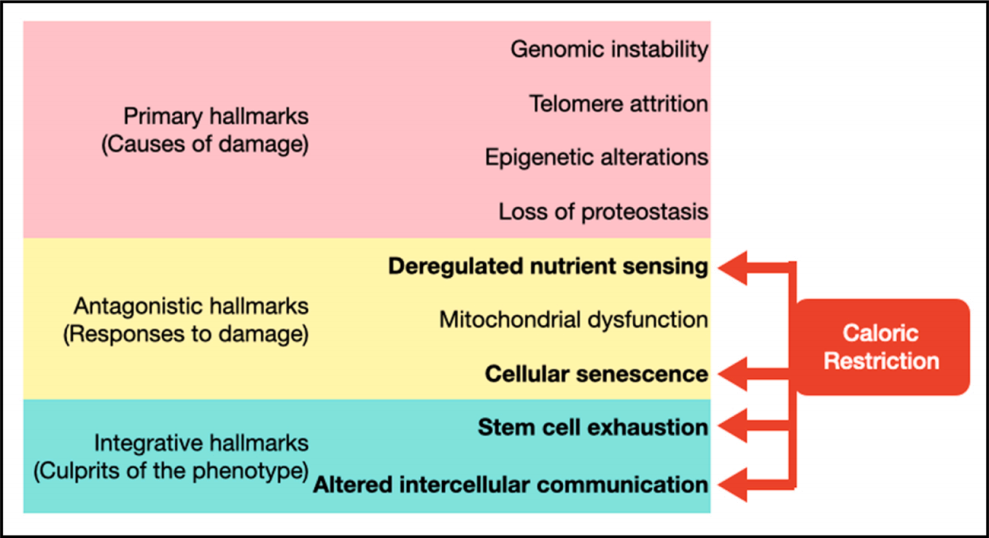
\includegraphics[width=0.8\textwidth]{cr_pathway_effects} \\
    Source: \cite{erbaba2020effects} \\
    \pause
    Extension: about 20-40\% QUALY \cite{swindell2012dietary} \\
    \pause
    \textbf{State: In clinical trial}, e.g. \cite{TAMETarg47:online}
\end{frame}


\subsection{Senolytics}

\begin{frame}[c]{Senescent Cells}
    \large

    \begin{itemize}[<+(1)->]
        \item Send out Senescence-Associated Secretory Phenotype (SASP)
        \item SASP causes inflammation and age-related diseases, e.g. Arthritis, Atherosclerosis
        \item Cells induce apoptosis (suicide) or wait to get removed by immune system
        \item About 8\% of cells in young, and 17\% of cells in old mice are senescent \cite{folgueras2018mouse}
    \end{itemize}
\end{frame}

\begin{frame}[c]{Senescent Cell Effects}
    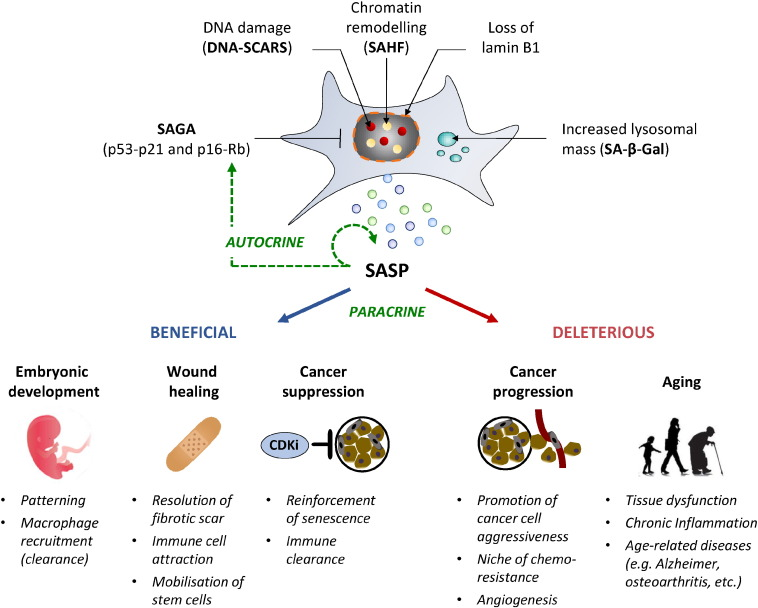
\includegraphics[height=0.85\textheight]{sasp_effects} \\
    Source: \cite{malaquin2016keeping}
\end{frame}


\begin{frame}<handout>[c]{Inflammation Effects}
    \begin{aquote}{\cite{NintilTh68:online}}
        {\em Also, the environment that inflammation creates is one that is} meant to
        increase cell turnover {\em (More apoptosis, but also more cell growth to
        replace lost cells), with granulocytes secreting toxic agents
        (Including ROS) to make the area affected less hospitable (But also
        increases damage to DNA), and specific cytokines like the} tumor
        necrosis factor that induce cell death, and growth factors that promote
        cell growth.
    \end{aquote}
\end{frame}

\begin{frame}[c]{Senolytics: Uses and Effects} 
    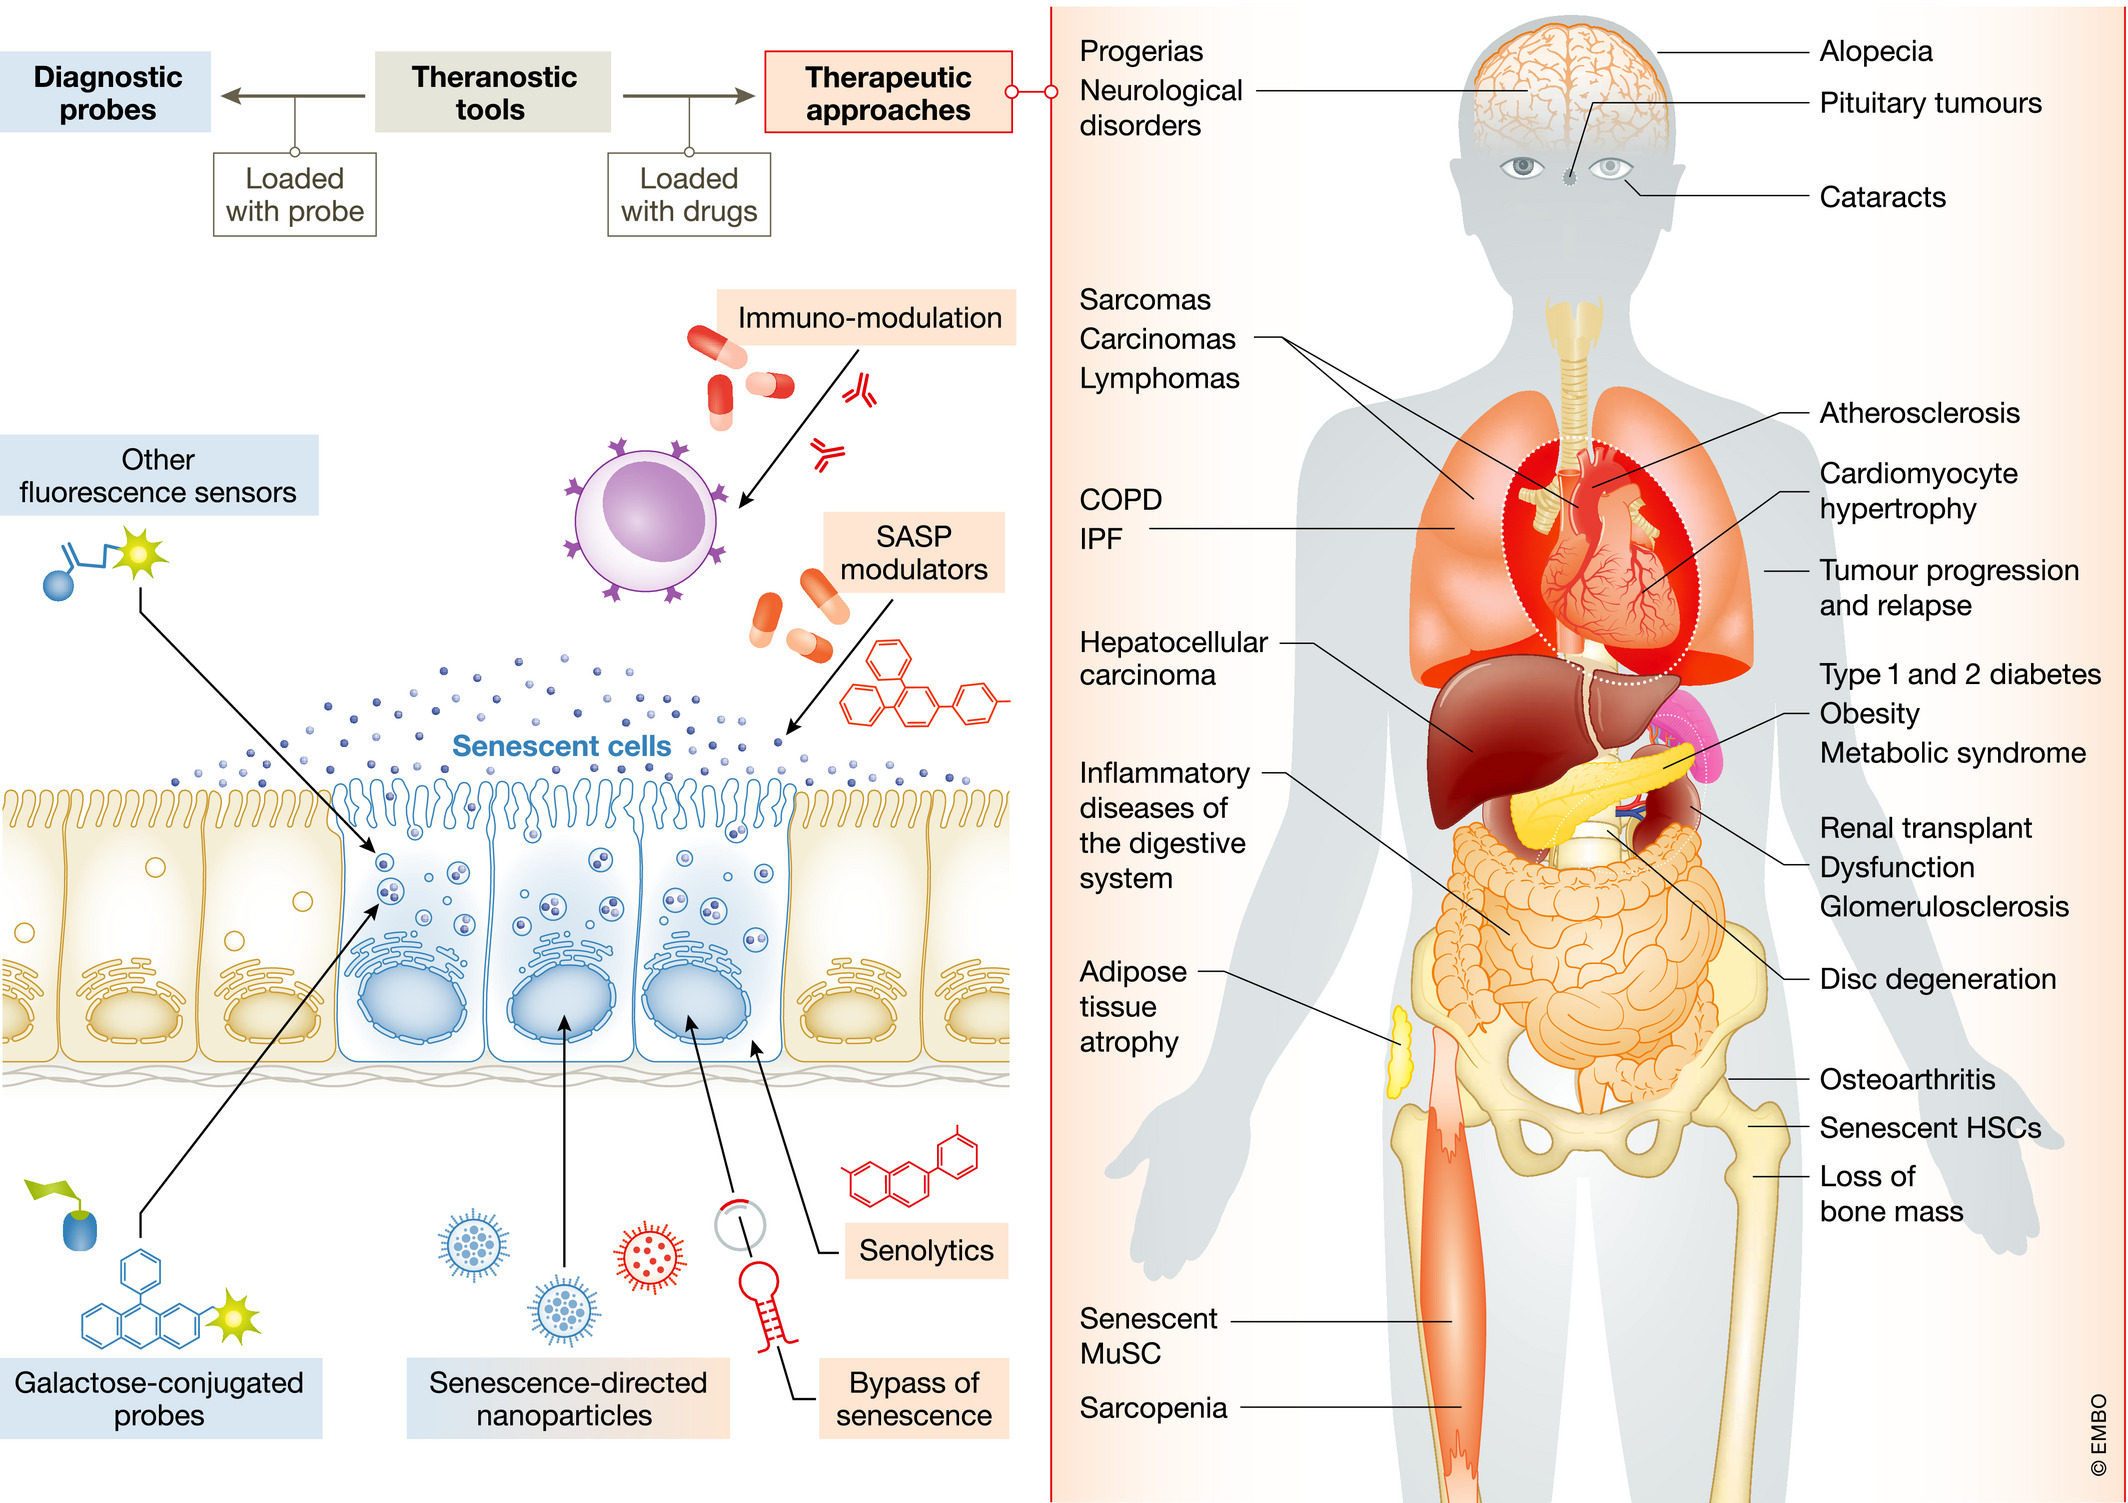
\includegraphics[height=0.85\textheight]{senescent_strategies} \\
    Source: \cite{paez2019targeting}
\end{frame}

% \begin{frame}[c]{Senolytics (Drugs killing senescent cells)}
%     Senescent cells are a kind of 'zombie'-like cell that accumulate with age. They are death-resistant cells that secrete proinflammatory factors associated with a range of age-related diseases (below, right):
% 
% Cellular senescence is associated with multiple human disorders. The development of galactose‐conjugated and fluorescent probes to detect and highlight senescent cells offers an important opportunity for longitudinal monitoring of senescence in clinical trials. Pharmacologically active small compounds known as senolytics inhibit pro‐survival pathways in senescent cells leading to apoptosis, a therapeutic strategy that may additionally be enhanced by the use of immune modulators promoting natural clearance of senescent cells. Finally, nanoparticles encapsulating cytotoxic drugs, tracers and/or small molecules can be used as theranostic tools, both for therapeutic and diagnostic purposes. Source: here
% There are various strategies being explored to kill or reprogram senescent cells (above, left), including senolytics. Senolytics are drugs that kill senescent cells to improve physical function and healthy lifespan. When administered to older mice, senolytics have been shown to reverse many aspects of aging such as cataracts, and arthritis (below):
% 
% Killing senescent cells with senolytics extends the median healthy lifespan by up to 27\% in mice (below). Several senolytics, such as the combination of dasatinib and quercetin, and fisetin are in clinical trials in humans today.
% 
% Study design for clearance of senescent cells mouse cohort. Median survival (in days, d) and percentage increase in median survival are indicated. Source: here
% Hallmarks of aging reversed: senolytics decelerate cellular senescence, improve epigenetic markers and restore intercellular communication (by reducing inflammation associated with senescent cells) to extend healthy lifespan.
% \end{frame}


\begin{frame}[c]{Method Evaluation: Senolytics}
    \textbf{Hallmarks affected}: \\
    \begin{itemize}[<+(1)->]
        \item Decelerate Cellular Senescence
        \item Improve Epigenetic Markers
        \item Restore Intercellular Communication (by reducing inflammation associated with senescent cells)
    \end{itemize}
    \pause
    Extension: 27\% median Life\\
    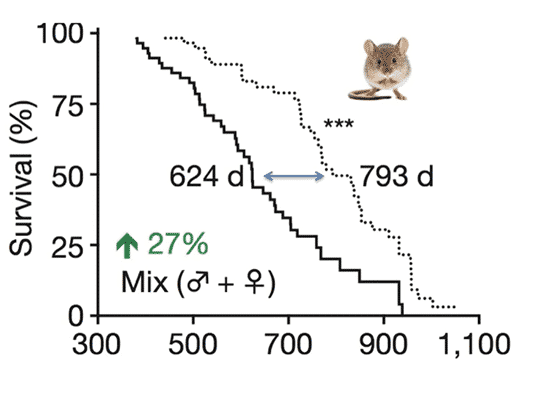
\includegraphics[width=0.4\textwidth]{senolytics_extend_life}
    Source: \cite{baker2016naturally} \\
    \pause
    \textbf{State: In clinical trial}
\end{frame}


\subsection{Cellular Reprogramming}

% \begin{frame}[c]{Cellular Reprogramming}
%     Cellular reprogramming is the conversion of terminally differentiated cells (old cells) into induced pluripotent stem cells (IPSCs) (‘young’ cells). Cells can be re-programmed to a youthful state using a cocktail of 4 factors known as Yamanaka factors, a finding for which a Nobel prize was awarded in 2012.
% 
% Induced pluripotent stem cells (IPSCs) have essentially unlimited regenerative capacity and carry the promise for tissue replacement to counter age-related decline. Partial reprogramming in mice has shown promising results in alleviating age-related symptoms without increasing the risk of cancer.
% 
% (A) The diagram depicts cellular programming to pluripotency, in other words, the conversion of terminally differentiated somatic cells into induced pluripotent stem cells (iPSCs) by cellular reprogramming through forced expression of Yamanaka factors (Oct4, Sox2, Klf4, and c-Myc). (B) The diagram depicts the rejuvenation of aged cells by cellular reprogramming. The process results in the amelioration of hallmarks of aging such as mitochondrial dysfunction, shortening of telomere length, changes in epigenetic marks, increased DNA damage, and senescence. Source: here.
% An impressive example of cellular reprogramming was the restoration of vision in blind mice with a severed optic nerve using 3 of the 4 Yamanaka factors. The researchers from Harvard Medical School were able to regrow a fully functioning optic nerve in mice using cellular reprogramming. This approach could be used in future to regenerate other tissues as a new anti-aging strategy.
% 
% Using the eye as a model tissue, expression of Oct4, Sox2 and Klf4 genes (OSK) in mice resets youthful gene expression patterns and the DNA methylation age of retinal ganglion cells, promotes axon regeneration after optic nerve crush injury, and restores vision in a mouse model of glaucoma and in normal old mice. Source: here.
% Hallmarks of aging targeted: Cellular reprogramming has been shown to reverse many of the hallmarks of aging, such as mitochondrial dysfunction, shortening of telomere length, changes in epigenetic marks, genomic instability, and cellular senescence.
% \end{frame}


\begin{frame}[c]{Method Evaluation: Cellular Reprogramming}
    \textbf{Hallmarks affected}: \\
    \begin{itemize}[<(1)->]
        \item Mitochondrial Dysfunction
        \item Shortening of Telomere length
        \item Changes in Epigenetic markers
        \item Genomic Instability
        \item Cellular Senescence
    \end{itemize}
    \pause
    Extension: \\
    \pause
    State:
\end{frame}



\subsection{Other Approaches}

\begin{frame}[c]{Other Approaches}
    Although not covered here, there are many other promising strategies for rejuvenation including thymic rejuvenation which has been shown to reverse biological age in humans, sirtuin enzyme activation with drugs such as resveratrol, and boosting mitochondrial function with NAD+ precursor molecules. All of these show the potential to increase healthy lifespan by targeting the hallmarks of aging.
\end{frame}


\begin{frame}[c]{Method Evaluation: Others}
    \textbf{Hallmarks affected}: ??? \\
    \pause
    Extension: ??? \\
    \pause
    State: Active Research
\end{frame}


